\section*{Modulazione Numerica in Banda Passante}

\subsection*{Segnale Passa Banda}

Il segnale passa banda può essere espresso come:
\[
    s(t) = a(t) \cos(2\pi f_0 t + \phi(t))
\]
dove \( a(t) \) è l'inviluppo reale di \( s(t) \) (segnale passa-basso) e \( \phi(t) \) la fase di \( s(t) \).



Possiamo scrivere \( s(t) \) come:
\[
    s(t) = \Re\left\{ a(t) e^{j[2\pi f_0 t + \phi(t)]} \right\}
\]
\[
    = \Re\left\{ a(t) \cos(2\pi f_0 t + \phi(t)) + j \ a(t) \sin(2\pi f_0 t + \phi(t)) \right\}
\]
\[
    = a(t) \cos(2\pi f_0 t + \phi(t)) = \Re\left\{ \tilde{s}(t) e^{j2\pi f_0 t} \right\}
\]
dove \( \tilde{s}(t) \) è l'inviluppo complesso di \( s(t) \) che quindi si definisce come:
\[
    \tilde{s}(t) \coloneqq a(t) e^{j\phi(t)}
\]

\paragraph*{PAM in banda passante}



% Definizione di M-PAM
La modulazione M-PAM si caratterizza per avere i seguenti simboli: \( A_s = \{\alpha_1, \alpha_2, \ldots, \alpha_M\} \),
dove ogni simbolo \( \alpha \) è definito come \( \alpha = 2i - 1 - M \).

L'impulso utilizzato per la trasmissione (TX) è rappresentato da \( p(t) \) e
il segnale modulato passa-banda \( s(t) \) è espresso come:
\[
    s(t) = \sum_{n=-\infty}^{\infty} x[n]\cdot p(t - nT_s)\cdot \cos(2\pi f_0 t).
\]

\begin{center}
    \begin{tikzpicture}[auto, node distance=2cm,>=latex']
        \tikzstyle{block} = [draw, rectangle, minimum height=2.5em, minimum width=4em]
        \node [input, name=input] {};
        \node [block, right of=input] (channel) {$p(t)$};
        \node [draw, circle, right of=channel] (sum) {\(\times\)};
        \node [output, right of=sum] (output) {};
        \node [below of=sum] (noise) {$\cos(2\pi f_0 t)$};

        \draw [->] (input) -- node {$x[n]$} (channel);
        \draw [->] (channel) -- node {} (sum);
        \draw [->] (noise) -- node {} (sum);
        \draw [->] (sum) -- node {$s(t)$} (output);
    \end{tikzpicture}
\end{center}


\[
    \tilde{s}(t) = \sum_{n=-\infty}^{\infty} x[n]\cdot p(t - nT_s)
\]
\[
    s(t) = \Re\{\tilde{s}(t) e^{j2\pi f_c t}\}
\]
\[
    = \Re \left\{ \sum_{n=-\infty}^{\infty} x(n) \cdot p(t - nT_s) \cdot e^{j2\pi f_c t} \right\}
\]
\[
    = \Re \left\{ \sum_{n=-\infty}^{\infty} x[n] \cdot p(t - nT_s) \cdot (\cos(2\pi f_0 t) + j \sin(2\pi f_0 t)) \right\}
\]

\[
    = \sum_{n=-\infty}^{\infty} x[n] \cdot p(t - nT_s) \cdot \cos(2\pi f_0 t)
\]

\begin{center}
    \begin{tikzpicture}[>=Stealth,
            block/.style={draw, rectangle, minimum height=2em, minimum width=3em},
            sum/.style={draw, circle, node distance=1cm},
            node distance=2cm and 3cm
        ]
        \draw[->] (-4,0) -- (4,0) node[below] {};

        \foreach \x in {-3,-2,-1,0,1,2,3}
        \draw (\x,0.1) -- (\x,-0.1) node[below] {$\x$};
        \foreach \x in {-3,-1,1,3}
        \fill[orange] (\x,0) circle (3pt);

        \node[below=0.75cm] at (0,0) {M=4};
    \end{tikzpicture}
\end{center}


\paragraph*{ Modulazione di fase PSK (Phase Shift Keying)}:

Definizione del segnale \(s_c(t)\):
\[
    s_i(t) = p(t) \cos(2\pi f_0 t + \theta_i) \quad \text{(simbolo \(i\)-esimo)}
\]
con
\[
    \theta_i = \frac{2\pi}{M}(i-1) \quad \text{per \(i = 1, \ldots, M\)}
\]

Espansione del segnale \(s(t)\) come sommatoria:
\[
    s(t) = \sum_{n=-\infty}^{\infty} p(t - nT_s) \cos(2\pi f_0 t + \theta[n])
\]
dove
\[
    \theta[n] \in A_s = \{\theta_1, \ldots, \theta_M\}
\]

\noindent Definizione del segnale modulato in fase $\tilde{s}_i(t)$:

\[
    \tilde{s}_i(t) = p(t) e^{j\theta_i}
\]
\[
    s_i(t) = \Re\{p(t) e^{j\theta_i} e^{j2\pi f_0 t}\} = \Re\{p(t) e^{j(2\pi f_0 t + \theta_i)}\} = p(t) \cos(2\pi f_0 t + \theta_i)
\]

\[
    x[n] = e^{j\theta[n]}
\]

\begin{equation*}
    s(t) = \Re \{ \tilde{s}(t) e^{j 2\pi f_0 t} \}
\end{equation*}
\begin{equation*}
    \tilde{s}(t) = \sum_{n=-\infty}^{\infty} e^{j \theta[n]} p(t-nT_s)
\end{equation*}

\begin{equation*}
    s(t) = \Re \left\{ \sum_{n=-\infty}^{\infty} p(t-nT_s) e^{j (2\pi f_0 t + \theta[n])} \right\}  = \sum_{n=-\infty}^{\infty} p(t-nT_s) \cos(2\pi f_0 t + \theta[n])
\end{equation*}


\begin{center}

    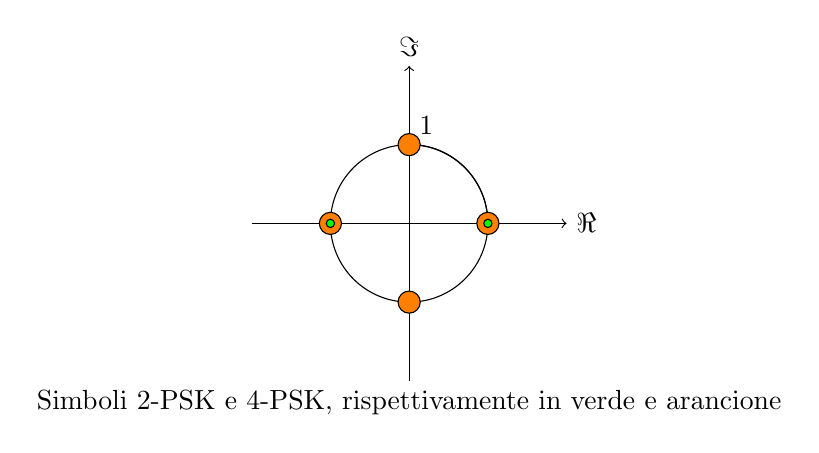
\begin{tikzpicture}
        \draw[->] (-2,0) -- (2,0) node[right] {$\Re$};
        \draw[->] (0,-2) -- (0,2) node[above] {$\Im$};
        \draw (0,0) circle (1cm);
        \draw[->] (1,0) arc (0:90:1cm);

        \draw (0,1) -- (0.1,1) node[above] {$\ \ 1$};

        \foreach \angle in {0, 90, 180, 270}{
                \draw[fill=orange] (\angle:1cm) circle (4pt);
            }
        \foreach \angle in {0, 180}{
                \draw[fill=green] (\angle:1cm) circle (1.5pt);
            }


        % insert caption here
        \node[below=2cm] at (0,0) {
            % in green 2-PSK, in orange 4-PSK, add caption
            % here
            Simboli 2-PSK e 4-PSK, rispettivamente in verde e arancione

        };


    \end{tikzpicture}

\end{center}
